\chapter{Optimizations}
\label{optimization}

Upon publishing $\plonk$ became a popular SNARK and variations of the protocol have been used in many cryptocurrency projects. This led to new improvements trying to make the protocol more efficient. The optimizations can be done on these three fronts:
\begin{enumerate}
    \item Polynomial commitment scheme 
    \item Interactive Protocol
    \item Recursive proof composition
\end{enumerate}

\paragraph{Polynomial commitment scheme} The $\plonk$ protocol was initially described with the KZG \cite{KZG} polynomial commitment schemes but other polynomial commitment schemes like \cite{FRI} could be used as well. As mentioned the MSM calculation in the polynomial commitments is a bottleneck in the prover algorithm, therefore making it more optimal might bring significant improvements. One of the authors of $\plonk$ already wrote a follow-up article constructing efficient polynomial commitment schemes for multiple points and polynomials \cite{shplonk} that can be used in $\plonk$.

\paragraph{Interactive protocol} This covers the rest of the protocol that is not about the polynomial commitment scheme. The possibilities range from more effective arithmetization to constructing more efficient polynomial checks. The major work in this area was done on using more complex custom gates and constructing lookup tables. When we limit the gates to only $+, \times$ for more complex programs the circuit size gets big. By being able to use custom gates we can enable better functionality and reduce the circuit size, which defines the complexity of the prover. These optimization techniques were described in \cite{turboplonk}. The lookup tables again authored by the same people that wrote $\plonk$ \cite{plookup} simply enable pre-compute values for some inputs $\publicinput$ and then prove that the witness $\witness$ exists in that table. These two approaches are independent of each other and can be combined with each other as was shown in the \cite{HyperPlonk}.

There are multiple approaches to optimizing the $\plonk$ protocol. Most of the heavy computations but the work of the verifier could be even more simplified by proof aggregation. The technique of recursive proof composition can aggregate several proofs into a single one. This makes the verification fast meaning all of the proof can be verified in one go. This has been used in \hl{xxx}. When optimizing one can try to make a more effective polynomial commitment scheme is the interactive oracle proof.

I have focused on the prover algorithm, specifically IOP. I led a discussion about the possible optimization with Tomáš Krňák who suggested looking at the interpolation and making it more effective. When running inverse Fourier transform the length of the vector needs to be a power of two. That is why the values are padded in the implementation. However, by reducing the degree of the wire polynomial we can also reduce the degree of the quotient polynomial and \hl{...}. 

\section{Degree reduction}
In my efforts, I have looked at the construction in the wire polynomials $a(x), b(x), c(x)$ and used \href{https://github.com/ZK-Garage/plonk}{PlonK implementation in ZK-Garage} as a reference implementation.

The implementation relies on the \href{https://github.com/arkworks-rs}{arkworks} library that implements $iFFT$ using the Cooley-Turkey algorithm that runs in time in time $\bigO{n\log{n}}$. This algorithm can interpolate only vectors of length that are powers of 2, which is why the polynomial is padded with zeros. However, this raises the degree of the polynomial. Lets 



\begin{figure}
    \centering
    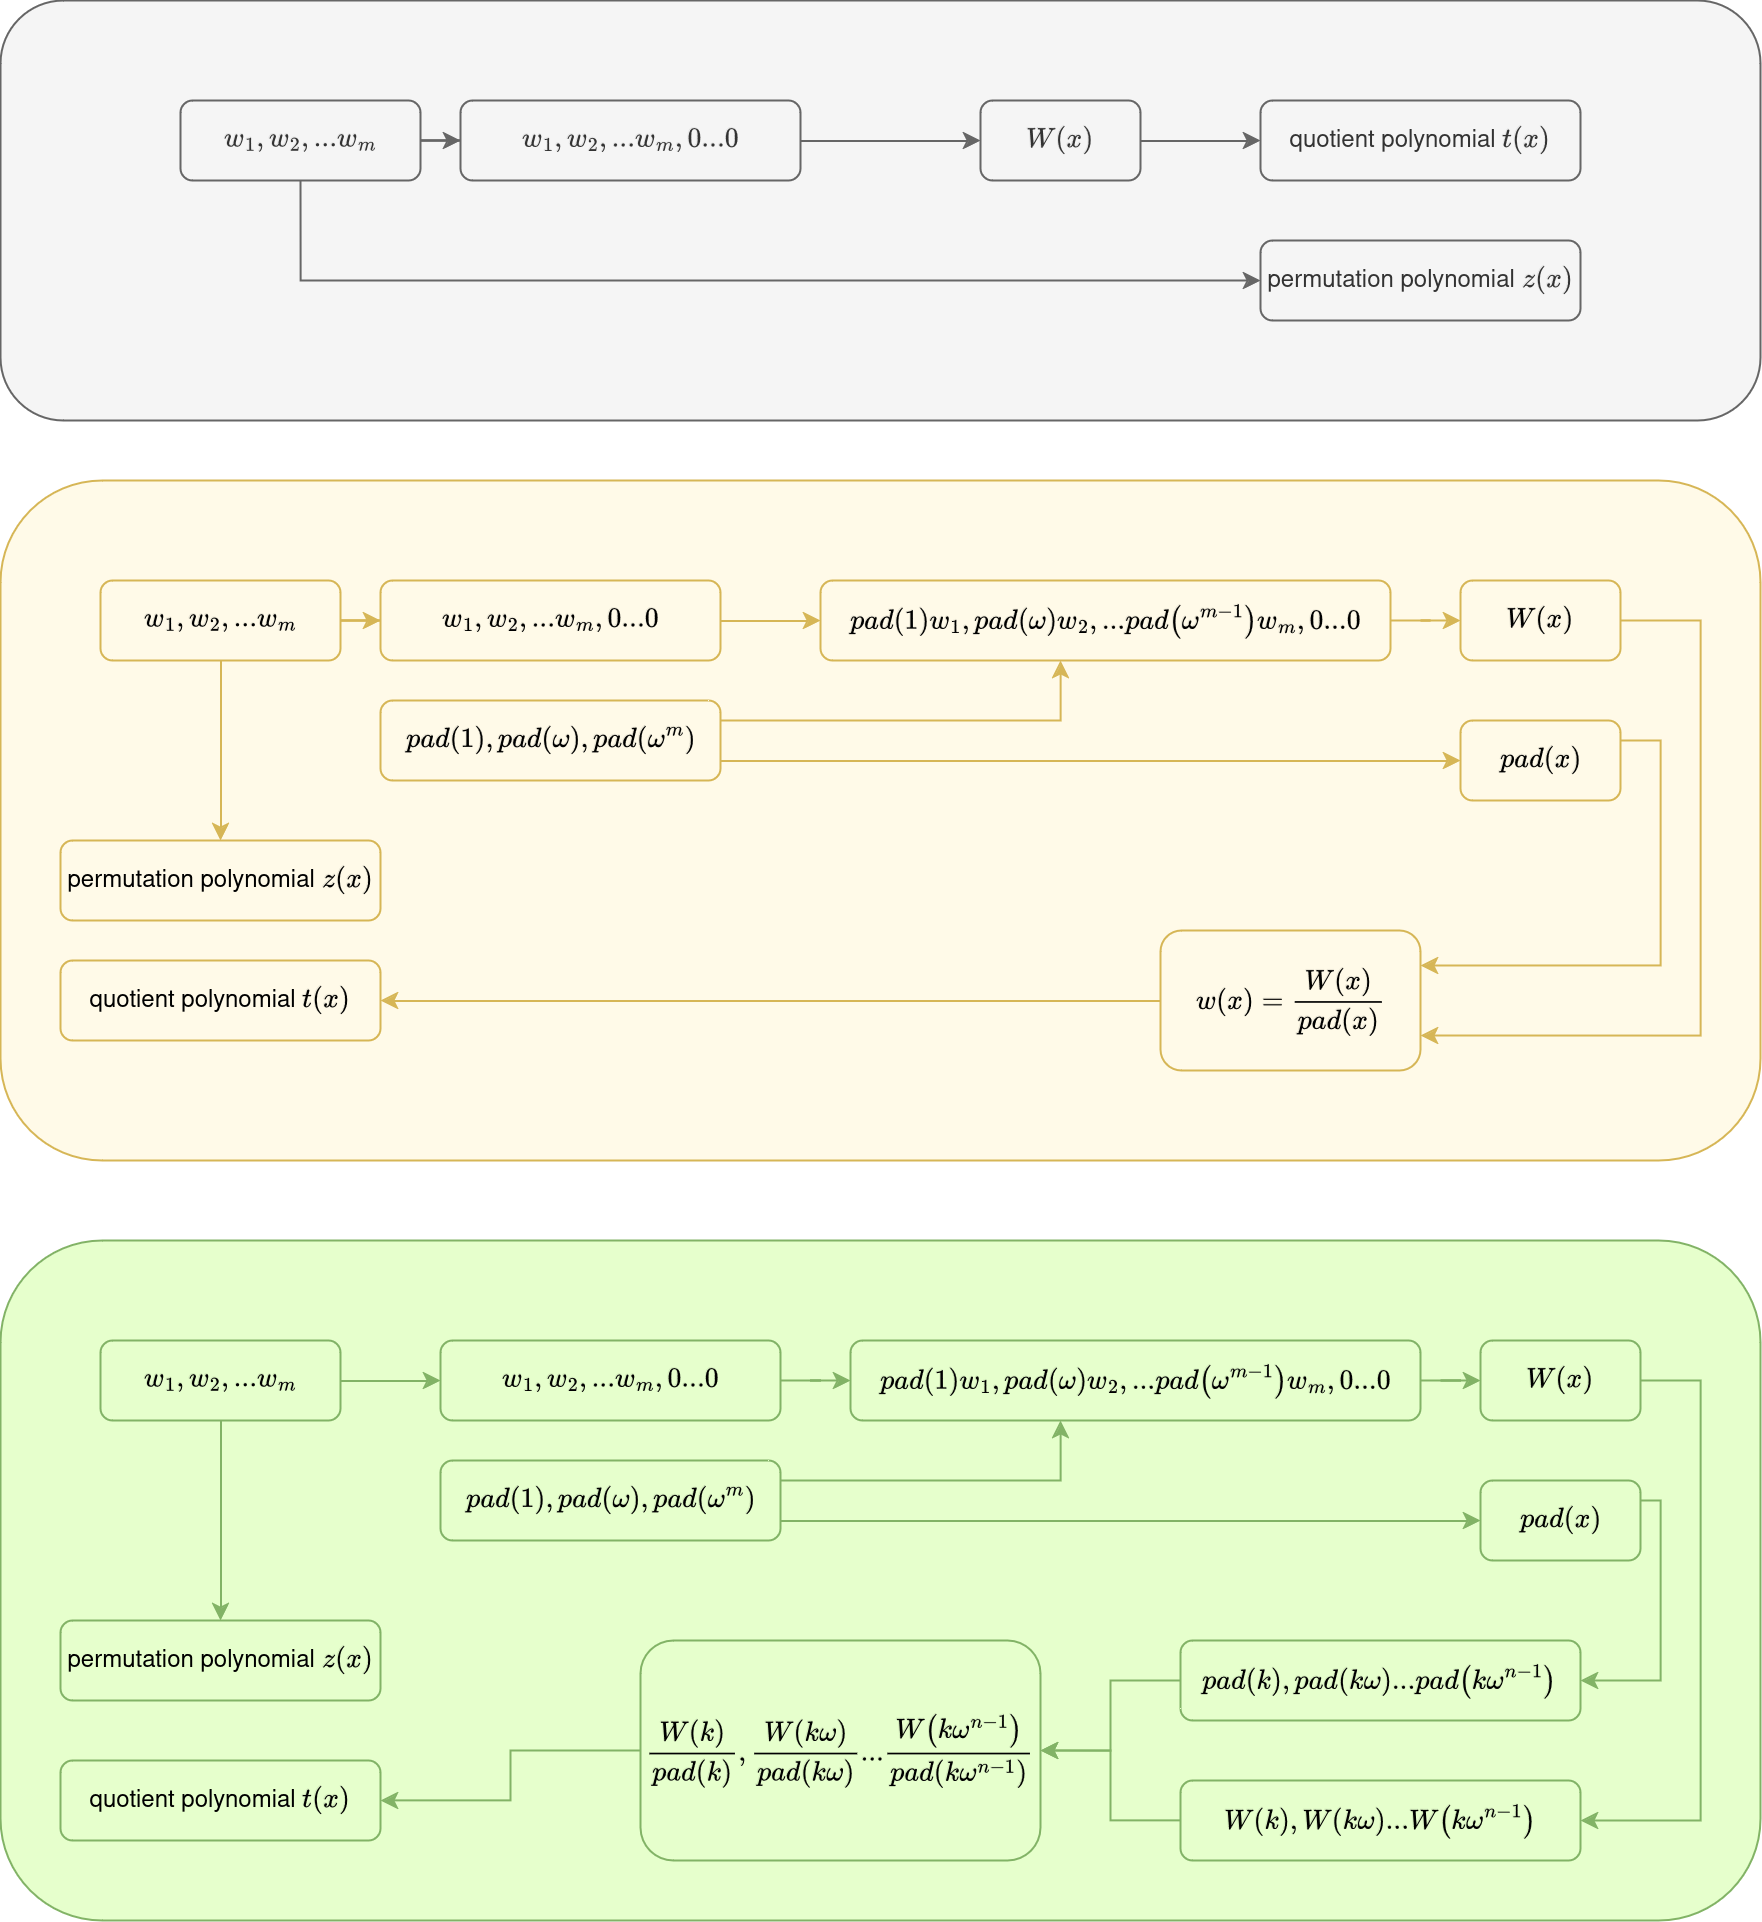
\includegraphics[width=1\linewidth]{figures/degree_reduction_diagram.drawio.png}
    \caption{Degree reduction variants}
\end{figure}

\section{Polynomial Division}
The standard polynomial division has complexity .... 
However, we can try to make the polynomial sparse and make it run faster.

\section{Pairwise division in the coset}
